\documentclass[letter]{scrartcl}

% Use UTF-8 encoding
\usepackage[utf8]{inputenc}
\usepackage{graphicx}

\title{Berlin -- The Pulse of a City}
\author{Tobias Gerken}
\date{\today}


\begin{document}

\maketitle

\section{Introduction}

According to  U.S.~Small Business Association \cite{SBA}, approximately 50\% of new businesses fail within five years of opening. Given the high risk and challenging retail environment, finding the right target demographic and business environment is therefore key. At the same time, cities are becoming increasingly dynamic and diverse which provides ample opportunities for business segmentation. 

Combining data-science approaches with the increasing availability of real time consumer data and open data from city governments can provide valuable insight that can businesses help attract and retain customers.  

\subsection{Business question}
Berlin, the capital of Germany, is home to approximately 3.6 million people and widely recognized to be one of Europe's most dynamic cities. 
Using the city of Berlin as example, we segment its districts by their population demographics and analyze what type of businesses thrive is the respective neighborhoods. The \emph{trending} feature of the Foursquare API, we analyze locations and neighborhoods in Berlin that are trending within a 24-h window letting us experience the \emph{Pulse of the City}.
\\

In detail we ask:
\begin{itemize}
\item Which neighborhoods have the highest density of trending venues?
\item Does the age distribution of district residents have a discernible impact on venues density and type?
\item Can we segment neighborhoods based on the type of business venues they attract and is there a relationship to the demographics Berlin's districts?  
\end{itemize}

\section{Data}

Berlin is a city state divided into 12 districts, each with populations between 200,000 and 400,000 (Figure\ref{fig:Berlin}).  

The Berlin state government provides demographics data for Berlin through its Open Data Portal \cite{Dem}. Geographic shape files of the Berlin districts \cite{Bez} and postcode \cite{PLZ} areas are available through the \emph{Technologie Stiftung Berlin} (Berlin Technology Foundation). 

\begin{figure}[h]
\centering
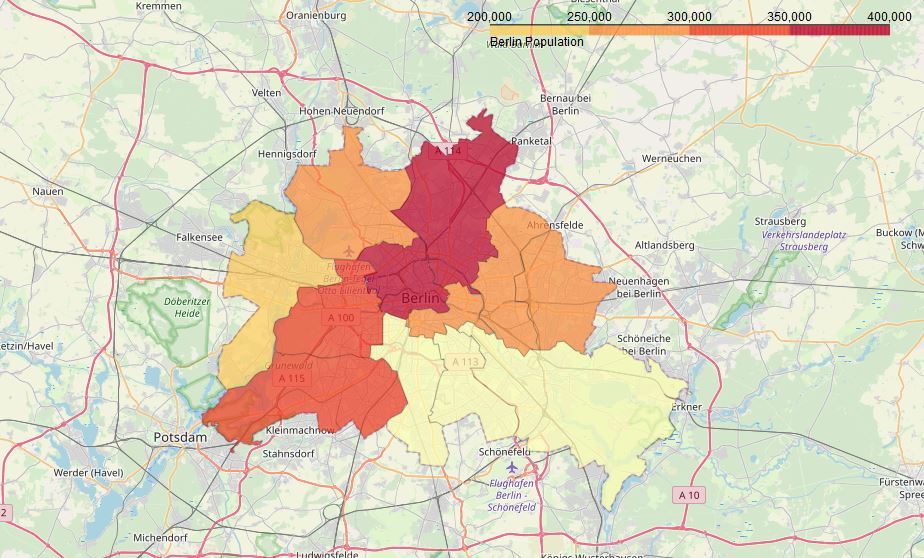
\includegraphics[width=12cm]{./Berlin_Pop.JPG}
\caption{Berlin is home to 3.6 million people, who live in 12 districts with 200,000 to 400,000 inhabitants each.}\label{fig:Berlin}
\end{figure}

Foursquare's API \cite{FS} allows to query business venue data based on geographical coordinates. Using the \emph{explore} functionality, we receive information about nearby venues, including their postcode and geographic coordinates, which allow them to be linked to Berlin's demographic data. The \emph{trending venues} functionality, allows us to find types of business venues and associated geographic areas that are popular during the course of a day. 

\subsection{Approach}

Demographic data at the city neighborhood-level (\emph{Ortsteil}) were downloaded in CSV-format and aggregated to district level. The demographic data is provided in age groups of 5 years. We suppose that similar age groups have similar consuption patterns and aggregated the data to age groups 0-15, 15-30, 30-50, 60-65, and over 60 years old (Table \ref{tab:demo}), approximately representing children, young adult, middle age, older, and senior consumers. 

\begin{table}[h]
\centering
\caption{There is considerable diversity in age group distribution between Berlin's districts. For example Friedrichshain-Kreuzberg has the larges share of middle age consumers, while Steglitz-Zehlendorf has a much older population.}
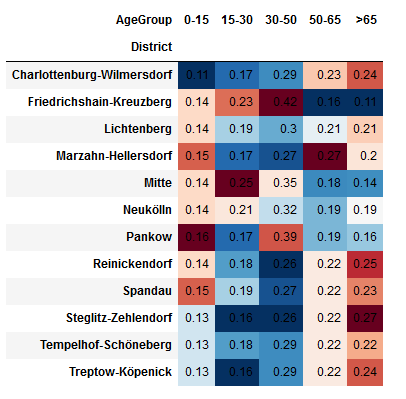
\includegraphics[width=10cm]{./BerlinTable_color.PNG}
\label{tab:demo}
\end{table}

To capture variation in business venues, we execute a gridded sampling approach (Figure \ref{fig:Grid}), where Berlin is covered with an equidistant grid of 2\,km length for which Foursquare search queries are being executed. The returned venues are aggregated by district and postcode area, retaining information about the nature of the business.   

\begin{figure}[h!]
\centering
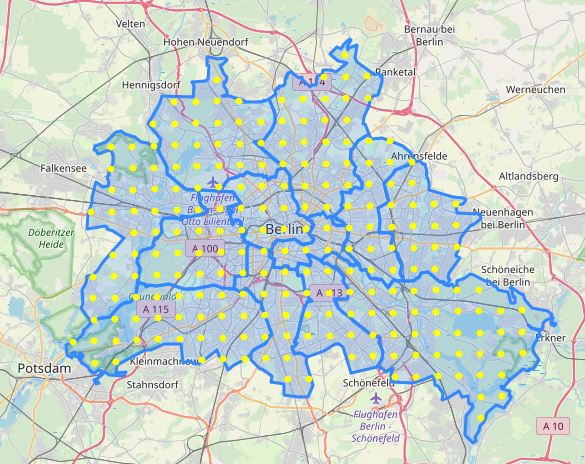
\includegraphics[width=12cm]{./Grid.JPG}
\caption{Sampling grid used for execution of the Foursquare venue explore functionality}\label{fig:Grid}
\end{figure}

\begin{thebibliography}{9}
  \bibitem{SBA} 
U.S.~Small Business Association: Do economic or industry factors affect business survival? 2012 \\
\texttt{https://www.sba.gov/sites/default/files/Business-Survival.pdf}, 
\bibitem{Dem}
Amt für Statistik Berlin-Brandenburg: Einwohnerinnen und Einwohner in den Ortsteilen Berlins am 30.06.2016, 2016 \\
\texttt{https://daten.berlin.de/datensaetze/einwohnerinnen-}
\texttt{und-einwohner-den-ortsteilen-berlins-am-30062016},   
 \bibitem{Bez}
 Technologiestiftung Berlin: Die Bezirksgrenzen der 12 Berliner Bezirke, 2017\\
 \texttt{https://data.technologiestiftung-berlin.de/dataset/bezirksgrenzen}  
  \bibitem{PLZ}
 Technologiestiftung Berlin: PLZ -- Postleitzahlgebiete Berlins, 2015\\
 \texttt{https://data.technologiestiftung-berlin.de/dataset/plz}
 \bibitem{FS}
 Foursquare Labs Inc: Places API, \texttt{https://https://developer.foursquare.com/docs}, Last Access: 4/28/2019
\end{thebibliography}

\end{document}